\section{Aufgabe 7 - Datenübertragung mittels Infra-Rot (IR)}
\label{sec:aufgabe-7---datenuebertragung-mittels-infra-rot-ir}

In dieser Aufgabe soll eine Datenübertragung mittels Infrarotsignal implementiert werden.
Um ein solches Signal in der verwendeten Simulationssoftware zu simulieren, wurde die Schaltung aus Abbildung \ref{fig:a7-simulation-infrarot} verwendet.

\begin{figure}
    \centering
    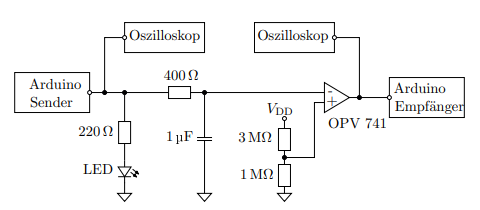
\includegraphics{pictures/a7-addon.png}
    \caption{Simulation eines Infrarotsignals}
    \label{fig:a7-simulation-infrarot}
\end{figure}

Für diese Aufgabe, soll ein 38kHz Signal von einem Sender-Mikrocontroller and einen Empfänger-Mikrocontroller gesendet werden.
Eine Übertragung von Text soll mithilfe des Sendens von Morsezeichen implementiert werden.
Es soll dem Benutzer dann ermöglicht werden, über die serielle Schnittstelle Zeichen an den Sender zu übergeben.
Dieser sendet die Zeichen dann an den Empfänger, welche sie wieder ausgibt.

\subsection{Materialien}
\label{subsec:a7-materialien}

\begin{table}[ht]
    \centering
    \caption{Aufgabe 7 - Verwendete Materialien}
    \label{tab:a7-materialien}
    \begin{tabular}{| l | l | l |}
        \hline
        Bezeichnung & Eigenschaften & Menge \\
        \hline
        LED & Rot & 1 \\
        Widerstand & $220\Omega$ & 1 \\
        & Rot - Rot - Braun - Gold & \\
        Widerstand & $400\Omega$ & 1 \\
        & Gelb - Schwarz - Braun - Gold & \\
        Widerstand & $1M\Omega$ & 1 \\
        & Braun - Schwarz - Grün - Gold & \\
        Widerstand & $3M\Omega$ & 1 \\
        & Orange - Schwarz - Grün - Gold & \\
        Kondensator & $10 \mu F$ - 1 \\
        Operationsverstärker & & 1 \\
        (optional) Oszilloskop & & 2\\
        Mikrocontroller & Arduino Uno R3 & 2 \\
        \hline
    \end{tabular}
\end{table}

\subsection{Vorbereitung}
\label{subsec:a7-vorbereitung}

\subsubsection{Aufgabe 1}

Zur Codierung von Buchstaben in Morsecode soll recherchiert werden, wie diese Codierung erfolgt.
Es werden sogenannte \textit{dit}s und \textit{dah}s verwendet \cite{morsecode}.
Ein \textit{dit} wird als Punkt und ein \textit{dah} als Strich symbolisiert.
Des weiteren wird nicht zwischen Groß- und Kleinbuchstaben unterschieden.
In Tabelle \ref{tab:a7-morsecode} werden die Zuordnung zwischen Buchstaben und Morsecode gezeigt.

\begin{table}[h]
    \centering
    \caption{Morsecode von Buchstaben}
    \label{tab:a7-morsecode}
    \begin{tabular}{| c | c | c | c | c | c |}
        \hline
        Buchstabe & Code & Buchstabe & Code & Buchstabe & Code \\
        A & * - & J & * - - - & S & * * * \\
        B & - * * * & K & - * - & T & - \\
        C & - * - * & L & * - * * & U & * * - \\
        D & - * * & M & - - & V & * * * - \\
        E & * & N & - * & W & * - - \\
        F & * * - * & O & - - - & X & - * * - \\
        G & - - * & P & * - - * & Y & - * - - \\
        H & * * * * & Q & - - * - & Z & - - * * \\
        I & * * & R & * - * & &  \\
        \hline
    \end{tabular}
\end{table}

\subsubsection{Aufgabe 2}

Es soll überlegt werden, wie das Einlesen von Zeichen und die Codierung dieser mittels eines Mikrocontroller efolgen könnte.

Zuerst kann ein Buchstabe mittels $Serial.read()$ eingelesen werden.
Durch die Verwendung einer Matrix, welche die Kodierung abbildet, kann ein Buchstabe kodiert werden.
Man kann dann ein Signal für die Dauer $t$ an einen Ausgangspin anlegen um ein dit zu senden.
Um ein dah zu senden, kann das Signal für die Dauer $3t$ anliegen.

\subsubsection{Aufgabe 3}

Es soll der benötigte Vorwiderstand der Infrarot-LED berechnet werden.
Dazu sind folgende Werte gegeben:

\begin{align}
    U = 5V \\
    I_D = 130mA \\
    U_D = 1,6V \\
    R_{on} = 14\Omega
\end{align}

\begin{figure}[h]
    \centering
    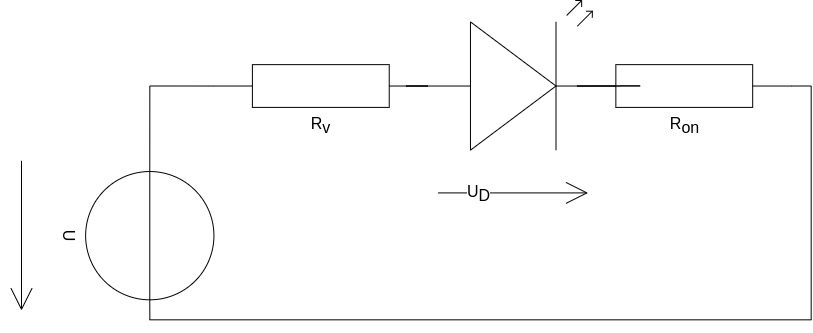
\includegraphics[height=0.3\textheight]{pictures/a7-rechnung-vorwiderstand.png}
    \caption{Angenommene Schaltung}
    \label{fig:a7-angenommene-schaltung}
\end{figure}

Gesucht ist der Widerstand $R_v$.
Zur Berechnung wurde die Schaltung aus Abbildung \ref{fig:a7-angenommene-schaltung} angenommen.

\begin{align}
    U_T = R_{on} * I_D \\
    = 14\Omega * 0,13A \\
    = 1,82V
\end{align}

\begin{align}
    U_{RV} = U - U_T - U_D \\
    = 5V - 1,82V - 1,6V \\
    = 1,58V
\end{align}

\begin{align}
    R_v = \frac{U_{RV}}{I_D} \\
    = \frac{1,58V}{0,13A} \\
    \underline{\underline{= 12,154\Omega}}
\end{align}

Der errechnete Vorwiderstand beträgt $12,154\Omega$, daher wird der $10\Omega$ Widerstand aus der E6-Reihe verwendet.

\subsection{Praktikumsaufgabe}
\label{subsec:a7-praktikumsaufgabe}

In Abbildung \ref{fig:a6-implementierung} ist die implementierte Schaltung abgebildet.


\begin{figure}
    \centering
    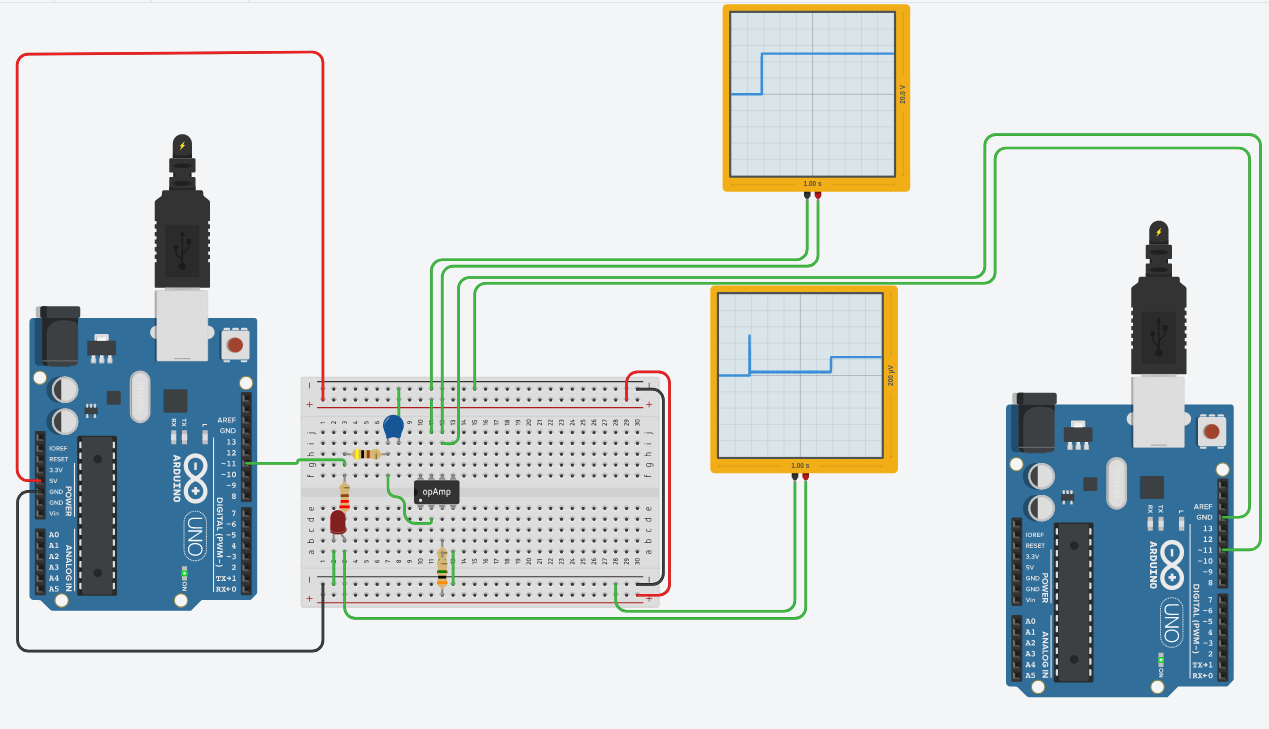
\includegraphics{pictures/a7-praktik.png}
    \caption{Implementierte Schaltung für Aufgabe 7}
    \label{fig:a7-implementierung}
\end{figure}


\subsection{Fehlerdiskussion}
\label{subsec:a7-fehlerdiskussion}

\subsection{Zusammenfassung}
\label{subsec:a7-zusammenfassung}
